\documentclass[12pt]{article}
\usepackage[english]{babel}
\usepackage[utf8x]{inputenc}
\usepackage{amsmath}
\usepackage{graphicx}
\usepackage{parskip}
\usepackage{ucs}
\usepackage{float}
\usepackage{array}
\usepackage{amsmath}
\usepackage{amssymb}
\usepackage{amsfonts}
\usepackage{latexsym}
\usepackage{graphicx}
\usepackage{caption}
\usepackage{ifpdf}
\usepackage{url}
\usepackage{xtab}
\usepackage{geometry}
\usepackage{longtable}
\usepackage{tabularx}
\usepackage{booktabs}
\usepackage[hidelinks]{hyperref}

\newcommand{\HRule}{\rule{\linewidth}{1mm}}
\parskip 7.0pt
\renewcommand{\baselinestretch}{1.5}
\begin{document}
\begin{titlepage}
\vspace*{\stretch{1}}
\noindent\HRule
\begin{center}
\huge
\noindent TDT4175 Information Systems \\ [7mm]
\large
\noindent\emph{\textbf{Group 19}}\\
\paragraph*{}
Bertrand Nils Mathieu Duquesnoy\\ 
Knut Aron Fludal\\
Michal Gačko\\ 
Lars Henrik Søreide Grytten\\
Agata Anna Jedryszek\\
Håvard Holmboe Lian \\
\end{center}
\noindent\HRule
\vspace*{\stretch{2}}
\end{titlepage}
\newpage
\pagenumbering{Roman} 
\tableofcontents
\newpage
\pagenumbering{arabic} 
\setcounter{page}{1}

%Input sections here
\chapter{Introduction}

Information is one of the most valuable resources of an organization. The NTNU’s information system is a computer-based information system, it is composed of several actors (figure \ref{fig:infsyscom})  that, put together, fill the role of an effective information system. However, the information doesn’t seem to be always easily accessible with the current NTNU’s information system.

The information system in the university is set up to help and to provide students with every kind of information they need. That is why the information must be accessible, accurate and complete. But, having good information is not enough, the system must be efficient, effective and have good performance standards to display properly and constantly the right information.

So, in order to avoid being misled by wrong information, the current system needs to be improved. The present report highlights some current problems and the solutions that can be brought.

\begin{figure}[H]
	\begin{center}
		\centerline{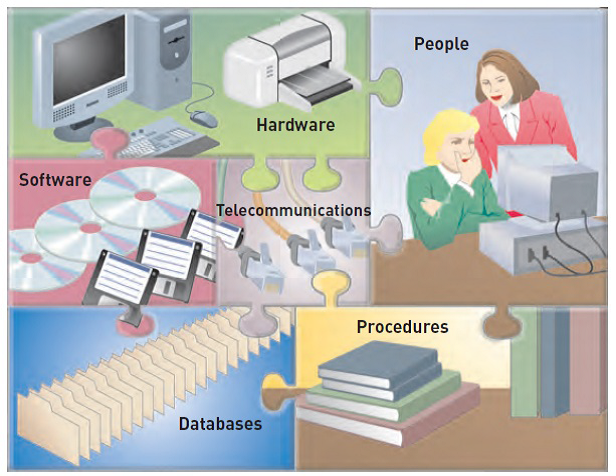
\includegraphics[scale=0.50]{infsyscom}}
		\caption[Computer-based information system components]{Computer-based information system components}
		\label{fig:infsyscom}
	\end{center}
\end{figure}

\section{Today's system}

The situation as it is today is that It's Learning, Examweb, and Student web are three separate systems with a common database on the back-end. 
This back-end system is called Felles Sudentsystem (FS) and powers many universities and univerity colleges in Norway.

%\subsection{It's Learning}
While Innsida is the main site for NTNU, It’s Learning main platform for students on a day-to-day basis. This is where all the information regarding courses they take are such as assignments, lecture slides, curriculum and last student assistant hours. This system also  where students deliver the assignments, receives feedback and grading on said assignments. 

It’s Learning is a system created by an external company, and is used widely as an teaching-platform among both high schools, universities and other higher educational institutes throughout the world. 

Since It’s Learning is a bought LMS, NTNU has very little say in the design and customization of the system. This has led many lecturers to creating their own systems, and using those instead. Example of this is most math-courses and TDT4120 (Algorithms and Datastructures).
%\subsection{Eksamensweb}

Eksamensweb is accessible from the innsida webpage. It gives everything you need to know about 
exams. The main webpage contains two parts. First, a static part giving contact details, location, 
postal address and examination regulations (i.e. such information as arrival time, calculators and 
dictionaries allowed and so on). Then a dynamic part containing 4 subparts listed below :

\subsubsection{Registration}

In this subpart you can check your exam dates, register for exams (you will be redirected on 
Studentweb to keep going over this task) and check about exam dates and locations. 
Also, you have information about the deadlines for registration for both semesters, about 
courses that have a "re-sit" or re-schedule exams and even if you need to register after the 
deadline (only special cases)
Below the previous section, there is insights about canceling your registration for exam in 
both semesters. This will also redirect you on Studentweb and you have to do it before the 
deadline otherwise you'll have to take the exam 


Final section is about special accommodations, this concerns you if you have health problem 
or a disability and then you can ask for special accommodations during your examinations. 
However, you will need to ask for it and there are deadlines for both semesters.

\subsubsection{Preparations}

This subpart permits you to deal with the organization of the exam. You can access reading 
rooms and study hall locations in order to study beforehand.
Then, you are given a link to courses information about date, time and room for you to know 
where and when to go and take your exam. If you lack specific information, you'll be 
redirected on Studentweb again for further details.
Finally, you can have details on previous examinations (organization details too) and how to 
master your examinations, that is to say getting help and improve your exam-taking skills and 
how examiners assess your work

\subsubsection{During examination}

This subpart deals with the very moment of the exam, it explains how the attendance works : 
you must arrive 10 minutes before the beginning of the examination, bring a photo 
identification and show this one to the invigilators before you can sign the attendance list.
You have a link that shows you the permitted examination aids, same link as the on in the 
static part of the webpage.
Then, some insights about how it is during the exam, if you are all of a sudden overwhelmed 
by some illness, if you ever try to cheat on an examination and some details on the presence 
of teaching staff during examinations.
Last section helps you to find the examination room. Indeed, it gives you a link of an 
overview of the lecture halls and rooms, a map of NTNU's campuses and the map of 
Trondheim Spektrum.

\subsubsection{Examination results}

Last subpart of the dynamic part, it deals with the results. It gives you the examination result 
deadline, the explanation of grades and appeals and grade scale. Once the results are posted 
online, you can check them on Studentweb.
You are also given a transcripts and diplomas/certificates details. Here you can order a 
transcript or diploma/certificate and you can also ask for a diploma supplement.
Last section concerns the new examination, if you ever need to retake an exam in order to 
improve your grade, you have the information you need. The very last point is about the re-
sit examination.
\subsection{Student web}

Student web is a portal where NTNU students can manage their course participation, register their personal information, check their grades, register in which faculty they wish to use their vote in student elections.
Studentweb is in use at NTNU and several other education institutions in Norway. It is developed by NTNU and the other institutions that make use of the system.

\end{document}